\documentclass[11pt]{article}
%ACENTOS
\usepackage[utf8]{inputenc}
\def\figurename{Fig.}
\def\tablename{Tabla}
\def\refname{Referencias}
\setlength{\parskip}{1em}

%PAQUETES
\usepackage{amsfonts,amsmath,amssymb}    % need for subequations
\usepackage{amsmath,latexsym}
\usepackage{graphics,color}
\usepackage{graphicx}
\usepackage{algpseudocode}
\usepackage[most]{tcolorbox}
\usepackage{hyperref} %Para colocar direcciones Web
\usepackage{booktabs} % Tablas
\usepackage[thinc]{esdiff} % Derivadas

%MARGEN
\setlength\topmargin{-0.5in}
\addtolength\oddsidemargin{-0.5in}
\setlength{\textheight}{23cm}
\setlength{\textwidth}{16cm}

%VARIABLES
\newcommand{\N}{\mathbb N}
\newcommand{\Z}{\mathbb Z}
\newcommand{\R}{\mathbb R}
\newcommand{\C}{\mathbb C}
\providecommand{\norm}[1]{\lVert#1\rVert}
%COLORES
\newcommand{\rojo}[1]{\textcolor[rgb]{1.00,0.00,0.00}{#1}}
\newcommand{\azul}[1]{\textcolor[rgb]{0.00,0.00,1.00}{#1}}
\usepackage{empheq}

\documentclass[fleqn]{article}
\usepackage{amsmath}

\newcommand{\cajaverde}[2]{
    \begin{tcolorbox}[colframe=green!70!black, title=#1]
        % Contenido
        #2
    \end{tcolorbox}
} 
  
\begin{document}

\begin{center}
 \Large \underline {\\ \\Tarea 6: Diferenciación e Integración numérica}
  \\
  \\
 \small  {Elaborado por Giselt Parra}\\ 
 \footnotesize{Vieres, 04 de Diciembre de 2020.}
\end{center}

\begin{center}
    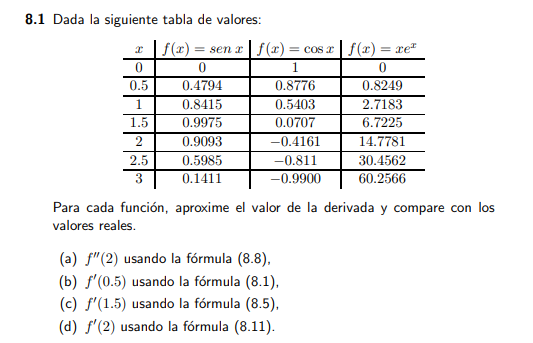
\includegraphics[keepaspectratio, width=12cm]{S1.png}
    \caption{\\}
\end{center} 


\vspace{0.5cm}
(a) Para $h = 0.5$ y $x=2$
\begin{equation}
  f''(x) = \frac{f(x + h) - 2f(x) + f(x - h)}{h^2} \hspace{1cm} 
\end{equation}

• \sin{x}

\\Valor real =  -0.41614  

\\ Valor aproximado = $\frac{\sin{2.5} - 2\sin{2} + \sin{1.5}}{0.5^2} = -0.89051$

\\ Error = 0.47437

• \cos{x}

\\Valor real = -0.90929  

\\ Valor aproximado = $\frac{\cos{2.5} - 2\cos{2} + \cos{1.5}}{0.5^2} = 0.40754$

\\ Error = 1.31683

• $xe^x$

\\Valor real = 22.16716  

\\ Valor aproximado = $\frac{{2.5}e^{2.5} - 2{2}e^{2} + {1.5}e^{1.5}}{0.5^2} = 30.49017 $

\\ Error = 8.32301


\vspace{0.5cm}
(b) Para $h = 0.5$ y $x=0.5$
\begin{equation}
 \frac{f(x + h) - f(x)}{h}
\end{equation}

• \sin{x}

\\Valor real =  0.87758  

\\ Valor aproximado = $\frac{\sin{1} - \sin{0.5}}{0.5} = 0.72409$

\\ Error = 0.15349

• \cos{x}

\\Valor real = - 0.47942

\\ Valor aproximado: $\frac{\cos{1} - \cos{0.5}}{0.5} = -0.67456$

\\ Error = 0.19514

• $xe^x$

\\Valor real = 2.47308  

\\ Valor aproximado = $\frac{e^1-0.5e^0.5}{0.5}= 3.78784 $

\\ Error = 1.31476

\vspace{0.5cm}
(c) Para $h = 0.5$ y $x=1.5$
\begin{equation}
 \frac{f(x + h) − f(x - h)}{2h}
\end{equation}

• \sin{x}

\\Valor real =  0.07073  

\\ Valor aproximado =  $\sin(2) − \sin(1) = 0.06782$

\\ Error = 0.00291

• \cos{x}

\\Valor real = -0.99749

\\ Valor aproximado = $\cos(2) − \cos(1) = -0.95644$

\\ Error = 0.04105

• $xe^x$

\\Valor real = 11.20422  

\\ Valor aproximado = $2e^2 - e = 12.05983 $

\\ Error = 0.85561


\vspace{0.5cm}
(d) Para $h = 0.5$ y $x=2$
\begin{equation}
 \frac{8f(x + h) - 8f(x - h) - f(x + 2h) + f(x - 2h)}{12h}
\end{equation}

• \sin{x}

\\Valor real = -0.41614 

\\ Valor aproximado =  $\frac{8\sin(2.5) - 8\sin(1.5) - \sin(3) + \sin(1)}{6}= -0.41530$

\\ Error = 0.00084

• \cos{x}

\\Valor real = -0.90929

\\ Valor aproximado = $\frac{8\cos(2.5) - 8\cos(1.5) - \cos(3) + \cos(1)}{6} = -0.90745$

\\ Error = 0.00184

• $xe^x$

\\Valor real = 22.16716 

\\ Valor aproximado = $\frac{8(2.5)e(2.5) - 8(1.5)(1.5) - (3)e(3) + e}{6} =22.05521$

\\ Error = 0.11195


%                       ENUNCIAR
%%%%%%%%%%%%%%%%%%%%%%%%%%%%%%%%%%%%%%%%%%%%%%%%
\vspace{1cm}
\begin{center}
    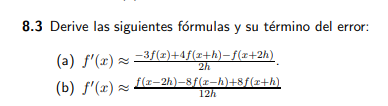
\includegraphics[keepaspectratio, width=10cm]{S2.png}
    \caption{\\}
\end{center} 

Las siguientes derivaciones fueron realizas por medio de polinomios interpolantes donde 

$$f'(x) = L'_0 f(a) + L'_1 f(b) + ... + L'_n f_n$$

donde las derivadas $L'_i$ son los coeficientes para la evaluación de la funciòn en los puntos correspondientes.

Para el calculo del error se toma en cuenta el teorema del error en la interpolación donde se anuncia que para cada $x \in [a, b]$ existe un núumero $\varepsilon \in (a, b)$ tal que

\begin{equation}
 f(x) - P(x) = \frac{f^{(n)}(\varepsilon)}{n!}\prod_{i=1}^n(x - x_i)
\end{equation}

Derivando y despejando $f'(x)$ en (5) tenemos
\begin{equation}
 f'(x) = P'_n(x) + \frac{f^{(n+1)}(\varepsilon)}{(n+1)!}\prod_{i=1}^n(x - x_i)
\end{equation}


(a) Para $a = x$, $b = x+h$, $c = x+2h$ derivar $f'(x) \approx \frac{-3f(x) + 4f(x+h) - f(x+2h)}{2h}$$

Tomando en cuenta dos puntos hacia delante y el valor a hallar debemos construir 


\begin{equation}
 f'(x) = L'_0 f(a) + L'_1 f(b) +L'_2 f(c)
\end{equation}

\vspace{0.25cm}
•$$L_0(x) =  
\frac{(x-b)(x-c)}{(a - b)(a - c)} 
$$
$$L_0'(x) =  
\frac{((x-b)(x-c))'}{-2h^2} = \frac{2x -c - b}{-2h^2}  = \frac{2x - x -2h - x - h}{-2h^2}  = \frac{-3}{2h}
$$

\vspace{0.25cm}
•$$L_1(x)  =  
\frac{(x-a)(x-c)}{(b - a)(b - c)} 
$$
$$L_1'(x)  =  
\frac{((x-a)(x-c))'}{-h^2} = \frac{2x - a - c}{-h^2}  = \frac{2x - x - x - 2h}{-h^2}  = \frac{2}{h} = \frac{4}{2h} 
$$


\vspace{0.25cm}
•$$L_2(x)  = 
\frac{(x-a)(x-b)}{(c - a)(c - b)}
$$
$$L_2'(x)  = 
\frac{((x-a)(x-b))'}{2h^2} = \frac{2x - a - b}{2h^2}  = \frac{2x - x - x - h}{2h^2}  = \frac{-1}{2h}
$$

Para el cálculo del error

$$E_2 =
\frac{f^{(3)}(\varepsilon)}{3!}((x-a)(x-b)(x-c))' = \frac{f^{(3)}(\varepsilon)}{3!}(3x^2-2ax-2cx-2bx+ac+cb+ab)' $$
$$= \frac{f^{(3)}(\varepsilon)}{3!}(3x^2-2(x+2h)x-2(x+h)x-2(x)x+(x+2h)(x+h)+(x+2h)(x)+(x+h)(x)) =
\frac{f^{(3)}(\varepsilon)}{3!}2h^2$$
Sustituyendo en (7) nos queda 
$$f'(x) \approx L_0' f(a) + L_1' f(b) + L_3' f(c) = \frac{-3f(x) + 4f(x+h) - f(x+2h)}{2h} + \frac{f^{(3)}(\varepsilon)}{3!}2h^2$$

\vspace{0.5cm}
(b) Para $a = x-2h$, $b = x-h$, $c = x+h$, $d = x+2h$  derivar $f'(x)  \approx \frac{f(x-2h) -8f(x+h) + 8f(x+h) - f(x+2h)}{12h} $

Tomando en cuenta dos puntos hacia delante, dos hacia atrás y el valor a hallar debemos construir 

\begin{equation}
 f'(x) = L'_0 f(a) + L'_1 f(b) +L'_2 f(c) + L'_2 f(d)
\end{equation}


\vspace{0.25cm}
•$$L_0(x) =  
\frac{(x-b)(x-c)(x-d)}{(a - b)(a - c)(a - d)} 
$$
$$L_0'(x) =  
\frac{((x-b)(x-c)(x-d))'}{-12h^3} = \frac{3x^2-2bx-2cx-2dx+bc+cd+bd}{-12h^3}  = \frac{-h^2}{-12h^3} = \frac{h}{12h} 
$$

\vspace{0.25cm}
•$$L_1(x)  =  
\frac{(x-a)(x-c)(x-d)}{(b - a)(b - c)(b - d)} 
$$
$$L_1'(x) =  
\frac{((x-a)(x-c)(x-d))'}{6h^3} = \frac{3x^2-2ax-2cx-2dx+ac+cd+ad}{6h^3}  = \frac{-4h^2}{6h^3} = \frac{-4}{6h} = \frac{-8h}{12h} 
$$

\vspace{0.25cm}
•$$L_2(x)  =  
\frac{(x-a)(x-b)(x-d)}{(c - a)(c - b)(c - d)} 
$$
$$L_2'(x) =  
\frac{((x-a)(x-b)(x-d))'}{6h^3} = \frac{3x^2-2ax-2bx-2dx+ab+bd+ad}{6h^3}  = \frac{-4h^2}{-6h^3} = \frac{4}{6h} = \frac{8h}{12h} 
$$

\vspace{0.25cm}
•$$L_3(x)  =  
\frac{(x-a)(x-b)(x-c)}{(d - a)(d - b)(d - c)} 
$$
$$L_3'(x) =  
\frac{((x-a)(x-b)(x-c))'}{12h^3} = \frac{3x^2-2ax-2bx-2cx+ab+bc+ac}{12h^3}  = \frac{-h^2}{12h^3} = \frac{-1}{12h} 
$$

Se abstiene del calculo para el error en este item dado a problemas para culminar las operaciones algebráicas, sin embargo, al igual que el punto (a) se hace uso de la fórmula (6)


Sustituyendo en (8) nos queda 
$$f'(x) \approx L_0' f(a) + L_1' f(b) + L_3' f(c) + L_4' f(d) = \frac{f(x-2h) -8f(x+h) + 8f(x+h) - f(x+2h)}{12h} + E_3 $$

\vspace{0.5cm}
\begin{center}
    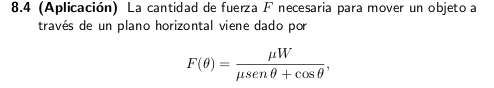
\includegraphics[keepaspectratio, width=12cm]{8.41.png}
    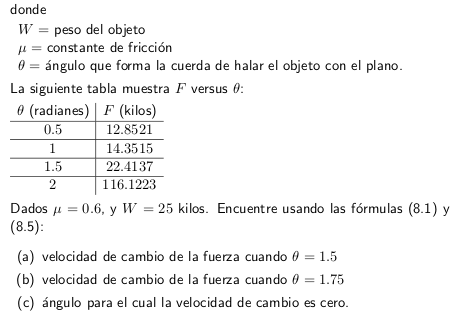
\includegraphics[keepaspectratio, width=12cm]{8.42.png}
\end{center} 

\vspace{0.25cm}
(a) Para $\theta$ = 1.5 

• Usando $\frac{f(x + h) - f(x)}{h}$ tenemos $\frac{f(2) - f(1.5)}{0.5} = 187.4172$

• Usando $\frac{f(x + h) − f(x - h)}{2h}$ tenemos $\frac{f(2) − f(1)}{2(0.5)} = 101.7708$

(b) Para $\theta$ = 1.75 

• $F(1.75) = \frac{15}{0.6\sin1.75+\cos1.75} = 36.39491$. Usando $\frac{f(x + h) - f(x)}{h}$ tenemos $\frac{f(2) - f(1.75)}{0.25} = 318.9$

• Usando $\frac{f(x + h) − f(x - h)}{2h}$ tenemos $\frac{f(2) − f(1.5)}{2(0.25)} = 187.4172$

(b) Para hallar el ángulo el cual la velocidad de cambio es cero desarrollaremos $\frac{f(x + h) − f(x - h)}{2h}$ con $x = \theta$
\begin{equation}
 F'(\theta) \approx	\frac{F(\theta+h)-F(\theta-h)}{2h} = 0 = F(\theta+h)-F(\theta-h)
\end{equation}

$F(\theta+h) = \frac{15}{0.6\sin{\theta+h}+\cos{\theta+h}} = \frac{15}{0.6\sin{\theta}\cos{h}+0.6\cos{\theta}\sin{h}+\cos{\theta}\cos{h}-\sin{\theta}\sin{h}} $
con $h = \frac{\pi}{2}$ 

$\Rightarrow F(\theta+h) = \frac{15}{0.6\cos{\theta}-\sin{\theta}}$

Por otro lado, al desarrollar el término anterior con $h = \frac{\pi}{2}$  tenemos

$F(\theta-h) = \frac{15}{0.6\sin{\theta-h}+\cos{\theta-h}} =  \frac{15}{-0.6\cos{\theta}+\sin{\theta}}$

Al sustituir en la fórmula (9)

$F(\theta+h)-F(\theta-h) = \frac{15}{0.6\cos{\theta}-\sin{\theta}} - \frac{15}{-0.6\cos{\theta}+\sin{\theta}} = \frac{-9\cos{\theta}+15\sin{\theta}-9\cos{\theta}+15\sin{\theta}}
{(0.6\cos{\theta}-\sin{\theta})(-0.6\cos{\theta}+\sin{\theta})} $

$\Rightarrow \frac{-18\cos{\theta}+30\sin{\theta}}
{(0.6\cos{\theta}-\sin{\theta})(-0.6\cos{\theta}+\sin{\theta})} = 0$ 

$\Rightarrow -18\cos{\theta}+30\sin{\theta} = 0$ $\Rightarrow 18\cos{\theta} = 30\sin{\theta} $ $\Rightarrow \frac{18}{30} = \tan{\theta} $ $\Rightarrow \Artan{18}{30} = \Artan{\theta} $ $\Rightarrow  \theta= 0.54041 $

\begin{center}
    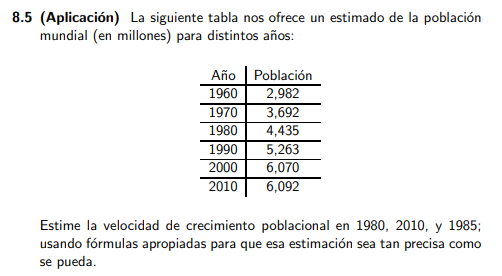
\includegraphics[keepaspectratio, width=12cm]{S4.png}
    \caption{\\}
\end{center} 

La estrategia para tomar las fórmulas más apropiadas consiste en escoger aquella que se adecue para poder tomar en cuenta el mayor número de puntos de la función que poseemos con respecto al valor de la velocidad de creimiento poblacional que queremos calcular.

• Para 1980, dado a que podemos tomar dos puntos hacia delante y hacia atrás se utilizará la fórmula  $\frac{f(x - 2h)  -8 f(x - h)+ 8 f(x + h) - f(x + 2h)}{12h}$ usando los años 1960, 1970, 1990 y 2000 dando como resultado $F'(1980) = 79$

• Para 2010, dado a que podemos tomar dos puntos hacia atrás y ese mismo año se utilizará la fórmula  $\frac{f(x - 2h)  -4f(x - h) + 3f(x)}{2h}$ usando los años 2010, 2000 y 1990 dando como resultado $F'(2010) = -74.1 $. Si analizamos los puntos de la tabla, a medida que pasan los años la población crece en cierta proporción, sin embargo, resulta llamativo lo pequeño de la diferencia que existe entre los años 2000 y 2010 considerando que ha pasado una década y dado al comportamiento que sigue este estudio se esperaría que el incremento fuera mayor. Al obtener una pendiente negativa se podría considerar posible que se haya llegado a un máximo comprendido entre esa década y que para 2010 la velocidad de crecimiento sea decreciente.

• Para 1985, dado a que podemos tomar dos puntos, uno hacia delante y otro hacia atrás siendo  la diferencia entre los años 5 se utilizará la fórmula  $\frac{f(x + h) − f(x - h)}{2h}$ usando los años 1980 y 1990 dando como resultado $F'(1985) = 82.8$

\begin{center}
    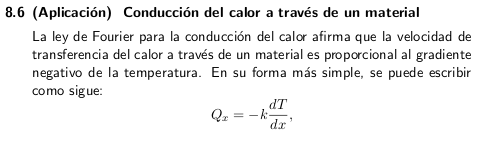
\includegraphics[keepaspectratio, width=12cm]{8.6.png}
    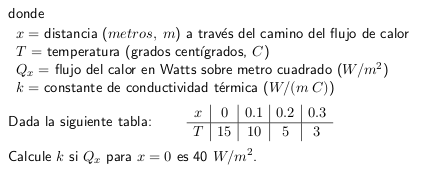
\includegraphics[keepaspectratio, width=10cm]{8.62.png}
\end{center} 

•$Q_x = -k \frac{dT}{dx}$
usando $ \frac{dT}{dx} \approx \frac{f(x + h) - f(x)}{h}$ y con $h = 0.1$, si $Q_x = 40 W/m^2$ para $x=0$ tenemos
$$40 = -k\frac{f(0.1) - f(0)}{0.1} = k50 \Rightarrow  k = \frac{50}{40} = 0.8$$

entonces el valor que cumple con estas condiciones es $k = 0.8 W/mC$

\begin{center}
    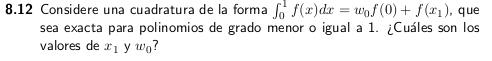
\includegraphics[keepaspectratio, width=12cm]{8.12.png}
    \caption{\\}
\end{center} 

Sabiendo que la cuadratura debe ser adecuada para polinomios de grado menos o igual a 1, se sabe que deriva de dos nodos para ser calculado. Esta caracteristica se cumple en la regla del trapecio y del rectangulo.

Considerando que la expresión dada está escrita como $w_0f(0)+f(x_1)$ que proviene de la forma $w_0f(x_0)+w_1f(x_1)$ entonces $w_1=1$ y $x_0=0$. Se descarta usar la regla del trapecio dado a que en ese caso $w_0 = w_1 = \frac{1}{2}$ tomando en cuenta que los lìmites de integracion van de [0,1]. 

La regla del rectángulo posee esta forma 
\begin{equation}
I_r = (b-a)[f(\frac{b+a}{2})]
\end{equation}
siendo $a=0$ y $b=1$ la expresión de arriba junto a la integral del enunciado queda como
$$ \int_{0}^{1} f(x)dx \approx I_r = f(\frac{1}{2})$$
y esto solo se cumple cuando $w0 = 0$ y $x_1 = \frac{1}{2}$ 

\vspace{0.5cm}
\begin{center}
    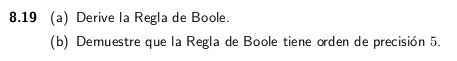
\includegraphics[keepaspectratio, width=12cm]{8.19.png}
    \caption{\\}
\end{center} 

Al igual que el cálculo del error en el item (b) del ejercicio 8.5, no se alcanzó llegar a la derivación de la regla mediante operaciones para ser plasmado explícitamente en el documento por lo extenso que resulta. No obstante, el camino por el cuál se pretendía llegar al resultado era mediante la integración de los polinomios interpolantes obtenidos con la base de Lagrange con cinco puntos. 

Teniendo todos los $L_i$ correspondientes y siendo la regla de Boole , sabemos que forma parte de las fórmulas de Newton-Cotes cuando $n=4$ por lo que se puede derivar de la siguiente forma

$$I_B = \int_b^a (L_0 f_0 + L_1 f_1 + L_2 f_2 + L_3 f_3)dx $$

con $f_i = f(x + ih)$ y $h= \frac{b-a}{4}$
\begin{center}
    
\includegraphics[keepaspectratio, width=12cm]{8.25.png}
    \caption{\\}
\end{center} 

$$\int_{0}^{x} f(t)dt \approx \frac{x}{6}[f(0)+4f(\frac{x}{2})+f(x)] = \frac{x}{6}[5+\frac{4x^9}{4608}+20x+20+\frac{x^9}{9}+10x+5] 
= \frac{43x^{10}}{2304} + 5x^2+ 5x$$

$$\Rightarrow \int_{0}^{x} f(t)dt \approx  \frac{43x^{10}}{2304} + 5x^2+ 5x = 11 $$

Se requiere una función de entrada para las iteraciones del método de Newton, para esto igualamos la expresión resultante en el paso anterior obteniendo asì que $g(x) = \frac{43x^{10}}{2304} + 5x^2+ 5x - 11$

\begin{tcolorbox}[colframe=blue!35!black, title=Código]
    IteracionesNewton.m
\end{tcolorbox}

Al ejecutar el programa con la función $g$, la raíz obtenida es $x = 1.0630$

\vspace{0.5cm}
\begin{center}
    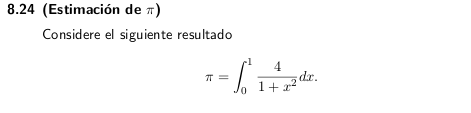
\includegraphics[keepaspectratio, width=12cm]{8.24.png}
    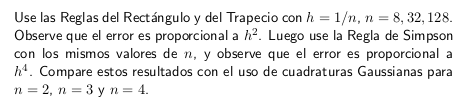
\includegraphics[keepaspectratio, width=12cm]{8.242.png}
    \caption{\\}
\end{center} 

\begin{tcolorbox}[colframe=blue!35!black, title=Código]
    ReglasVSCuadraturasGaussianas.m
\end{tcolorbox}

$$n = 8$$

• Por regla del rectángulo se obtuvo una aproximación de $\pi$ de 3.1429 con error 0.0013021.

• Por regla del trapecio se obtuvo una aproximación de $\pi$ de 3.1390 con error 0.0026042 siendo $h^2 = 0.015625$.

• Por regla de Simpson se obtuvo una aproximación de $\pi$ de 3.1416 con error 1.5113e-07 siendo $h^4 = 2.4414e-04$.

$$n = 32$$

• Por regla del rectángulo se obtuvo una aproximación de $\pi$ de 3.1417 con error 8.1380e-05.

• Por regla del trapecio se obtuvo una aproximación de $\pi$ de 3.1414 con error 1.6276e-04 siendo $h^2 = 9.7656e-04$.

• Por regla de Simpson se obtuvo una aproximación de $\pi$ de 3.1416 con error 3.6957e-11 siendo $h^4 = 9.5367e-07$.


$$n = 128$$

• Por regla del rectángulo se obtuvo una aproximación de $\pi$ de 3.1416 con error 0.82716.

• Por regla del trapecio se obtuvo una aproximación de $\pi$ de 3.1416 con error 1.0173e-05 siendo $h^2 =6.1035e-05$ .

• Por regla de Simpson se obtuvo una aproximación de $\pi$ de 3.1416 con error 9.7700e-15 siendo $h^4 = 3.7253e-09$.

\begin{center} Cuadraturas Gaussianas\end{center}

La regla para aproximar integrales por cuadraturas Gaussianas viene dada por
\begin{equation}
    \int_{-1}^{1} f(x)dx = \sum_{1}^{n}c_iP(x_i)
\end{equation}
definido en un intervalo [-1,1] y usando los valores $r_{n,i}$ como las raíces del polinomio. 
Dado a que la integral a aproximar posee distintos límites de integración que la igualdad expuesta, se debe proceder a hacer un cambio de variable $x = \frac{(b-a)t + a +b}{2}$ por lo que la formula a usar en las siguientes evaluaciones será

\begin{equation}
    \int_{0}^{1} f(x)dx = \int_{-1}^{1} \frac{1}{2}f(\frac{t+1}{2})dt =  \frac{1}{2}\sum_{1}^{n}c_{n,i}P(r_{n,i})
\end{equation}

$$n = 2$$
$$r_{2,1} = 0.5774, r_{2,2} = -0.5774, c_{2,1} = c_{2,0} = 1 $$
$$
G_2 = \frac{1}{2} [ \frac{4}{1+(\frac{0.5774+1}{2})^2} + \frac{4}{1+(\frac{-0.5774+1}{2})^2}] = 3.14753
$$
con un error de 0.00593.

$$n = 3$$
$$r_{3,1} = r_{3,3} = 0.7746, r_{3,2} = 0, c_{2,1} = c_{2,2} = 0.5556,c_{2,2} = 0.8889 $$
$$
G_3 = \frac{1}{2} [ \frac{4(0.5556)}{1+(\frac{0.7746+1}{2})^2} + \frac{4(0.8889)}{1+(\frac{1}{2})^2} +  \frac{4(0.5556)}{1+(\frac{-0.7746+1}{2})^2} ] = 3.14122
$$
con un error de 0.00037.

$$n = 4$$
$$r_{4,1} = -r_{4,4} = 0.8611, r_{4,2} = -r_{4,3} = 0.33998, c_{4,1} = c_{4,4}= 0.3478, c_{4,2} = c_{4,3} = 0.6521$$ 
$$
G_4 = \frac{1}{2} [ \frac{4(0.3478)}{1+(\frac{0.8611+1}{2})^2} + \frac{4(0.6521)}{1+(\frac{0.33998+1}{2})^2} + 
\frac{4(0.6521)}{1+(\frac{-0.33998+1}{2})^2} + \frac{4(0.3478)}{1+(\frac{-0.8611+1}{2})^2} ] = 3.14130
$$
con un error de 0.00029.

No se puede concluir que las reglas del trapecio rectángulo y Simpson aproximan mejor que usando cuadraturas Gaussianas dado a que la diferencia de segmentos generados es grande, sin embargo tomando en cuenta el resultado obtenido para n = 8 de las primeras reglas, el error en el peor caso resulta 0.0026042 mientras para $G_4$ el error resultante es 0.00029, esto quiere decir que por cuadraturas Gaussianas se obtuvo una mejor aproximación incluso cuando se usa la mitad de segmentos.

\vspace{0.5cm}
\begin{center}
    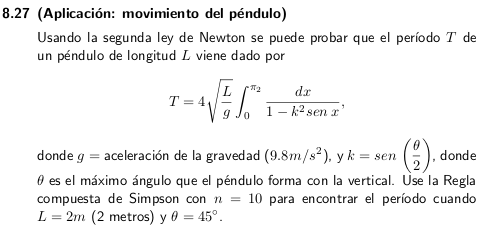
\includegraphics[keepaspectratio, width=12cm]{8.27.png}
    \caption{\\}
\end{center} 

$$\theta(radianes) = 0.7854$$
$$h = \pi/20$$

$$\int_{0}^{\pi/2} f(x)dx$$
$$\approx \frac{h}{3} [
f(0)+f(\pi/2)+4(f(h)+f(3h)+f(5h)+f(7h)+f(9h))+2(f(2h)+f(4h)+f(6h)+f(8h))]$$ 
$$= \frac{h}{3} [
2.17156+4(5.52929)+2(4.43776)] = \frac{h}{3}33.16424 = \frac{33.16424\pi}{60} = 1.73647
$$

Entonces $T = 4 \sqrt{\frac{2m}{9.8m/s^2}} 1.73647 = 3.13782s$


\vspace{1cm}	
%bibliografia
\begin{thebibliography}{9}

\bibitem{se} 
Ward Cheney y David Kincaid.
\textit{Numerical Mathematics and Computing, Sixth edition}.
The University of Texas at Austin.


\bibitem{fi} 
Richard L. Burden, J. Douglas Faires 
\textit{Numerical Analysis. NINTH EDITION}. 
Youngstown State University.

\bibitem{se} 
Biswa N. Datta, Luis M. Hernández-Ramos y Marcos Raydan.
\textit{Análisis Numérico. Teoría y Práctica}. 
[2018]

\end{thebibliography}
\end{document}
